\subsubsection{Experiments}
\label{sub:Experiments}
In order to determine the reliability of the hardware several experiments are conducted with the PIR sensor.
The tests are all based on data found in the datasheet for the hardware.
The main purpose of the tests is to determine the correlation between real world performance and the hardware specifications
found on the datasheet.
\\\\
Four tests are carried out with one main setup that are applied to all of them. The four consists of the following:

\begin{enumerate}
  \item Sensitivity Test
  \item Angle Test
  \item Distance Test
  \item Delay Time Test
\end{enumerate}
\subsubsection{The Setup}
\label{subs:The Setup}
As aforementioned the setup for all the experiments are identical
that is to ensure consistency of the results by reducing variables, that affects
the results, as much as possible.  The PIR sensor is placed in place surrounded wall
and where other moving objects are limited to a certain degree. In order to ensure that the
results are as precise as possible, all four tests are carried out at the same exact place but
the method of the individual test differs.
The PIR sensor is placed in a certain height and made sure the sensor itself is
sitting still during the tests.
\paragraph{Sensitivity}
\label{par:Sensitivity}

\subparagraph{Hypothesis}
\label{subp:SenHypothesis}
According to the datasheet the PIR sensor will be too sensitive if the distance potentiometer is rotated counter-clockwise.
The sensor should get so sensitivethat the PIR sensor would be triggered by the atmosphere even
if no moving object is existing\cite{datasheet_pir1}.
\subparagraph{Test Procedure}
\label{subp:SenTest Procedure}
The PIR sensor is configured with the distance potentiometer rotated
counter-clockwise as far as possible and the first triggered to test that everything works.
After the sensor is configured every object that can affect the sensor is
removed and the sensor is observed for 30 seconds.
The observation is to determine whether the sensor will detect objects that it is not
supposed to detect and how sensitive the sensor really can is.
\subparagraph{Results}
\label{subp:SenResults}

At the most sensitive setting, nothing was triggered by athmospheric noise. Just
to be sure, the sensor was tested at the least sensitive setting: nothing was
detected, as expected.

\subparagraph{Partial Conclusion}
\label{subp:SenPartial Conclusion}

According to our tests, the atmospheric noise was not detectable at the highest
sensitivity setting.

\paragraph{Angle}
\label{par:Angle}

\subparagraph{Hypothesis}
\label{subp:AngHypothesis}
According to the datasheet of the PIR sensor,
the sensor has a detecting angle of 120 degrees.
The sensor should according to the datasheet not detect any angle above 120 degrees.

\subparagraph{Test Procedure}
\label{subp:AngTest Procedure}
The sensor is placed in a certain position and detecting angle is measured equivalent to
the specified angle found in the datasheet.
For the sake of explanation let the angle above 120 degree be the grey zone and
the detecting area that is within the 120 degree white zone.
A moving object is placed in the grey zone and slowing moving into the white zone.
The PIR sensor should be triggered when the moving object enters the white zone in order
to work exactly as specified in the hardware specifications.
The zone of the moving object and PIR sensor is observed accordingly
and thereby the actual detecting angle is determined.

The test is performed three times on each side at the highest sensitivity of the sensor for consistency.

\subparagraph{Results}
\label{subp:AngResults}

run1 højre:
      97 y aksen
      79 x aksen
run1 venstre:
      81 y aksen
      50 x aksen
run2 højre:
      176 y aksen
      82 x aksen
run2 venstre:
      49 y aksen
      106 x aksen
run3 højre:
      174 y aksen
      88 x aksen
run3 venstre:
      65 y aksen
      108 x aksen


\subparagraph{Partial Conclusion}
\label{subp:AngPartial Conclusion}

\paragraph{Distance}

\subparagraph{Hypothesis}

According to the datasheet, the sensor can measure motion from 10 centimeters to
6 meters.

\subparagraph{Test procedure}

The sensitivity setting of the sensor essentially controls the distance. First,
the sensitivity is set to the lowest sensitivity. At that sensitivity, the
sensor should detect motion at a range of 10 centimeters, according to the above
hypothesis.

The sensor is measured by the test conductor approaching the sensor while
waving. Once the sensor detects the motion, the distance from the test conductor
to the sensor is measured. This is done three times to check for consistency. The sensitivity is then upped one unit on the sensor,
and the test conductor measures the distance for the new sensitivity.

\subparagraph{Results}

lowest sensitivity: < 10 centimeters
above + 1: < 10 centimeters
above + 1: 43 cm
above + 1: 123 cm
above + 1: 204 cm
above + 1: 245 cm (acted very strange, long beeps)
above + 1: 275 cm (acted very strange, long beeps)
above + 1: 413 cm
above + 1: 323 cm (acted strange, long beeps)
above + 1: 410 cm
above + 1: 547 cm
above + 1: 600 cm
above + 1: 515 cm

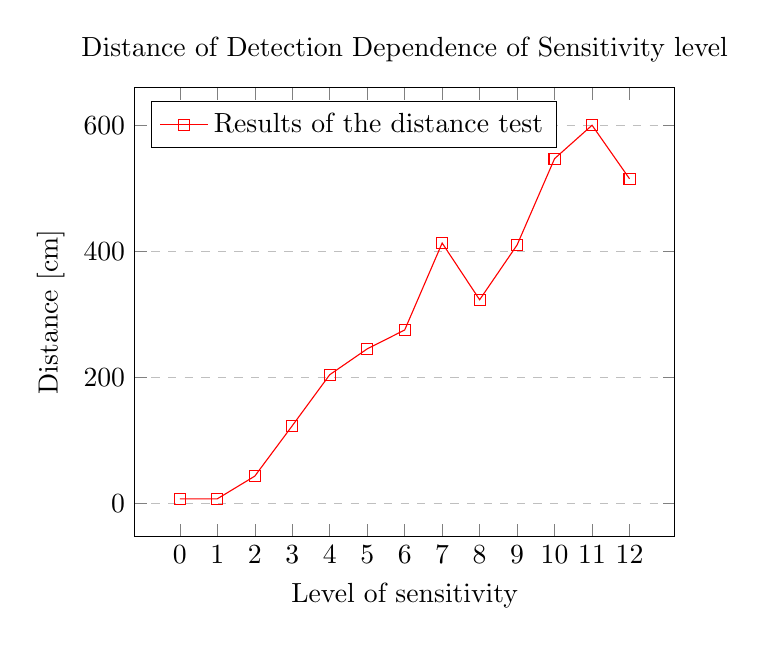
\begin{tikzpicture}
\begin{axis}[
    title={Distance of Detection Dependence of Sensitivity level},
    xlabel={Level of sensitivity},
    ylabel={Distance [cm]},
    %xmin=0, xmax=12,
    %ymin=0, ymax=120,
    xtick={0,1,2,3,4,5,6,7,8,9,10,11,12},
    %ytick={0,20,40,60,80,100,120},
    legend pos=north west,
    ymajorgrids=true,
    grid style=dashed,
]

\addplot[
    color=red,
    mark=square,
    ]
    coordinates {
    (0,7)(1,7)(2,43)(3,123)(4,204)(5,245)(6,275)(7,413)(8,323)(9,410)(10,547)(11,600)(12,515)
    };
    \legend{Results of the distance test}

\end{axis}
\end{tikzpicture}

\subparagraph{Partial conclusion}
The results indicates that there is a correlation between the sensitivity and the detecting distance.
However the sensor behave strange and unpredictable at sensitivity level 7 and 8.
Furthermore the sensor acted strange at sensitivity level 3, 4 and 5 by detecting something is was not supposed to detect.
However the maximum distance range seem to be 6meters as stated in the datasheet but at peak sensitivity level
the distance drops down to 5 meter only.

\paragraph{Delay time}

\subparagraph{Hypothesis}

According to the datasheet, the sensor has a delay time of 1 second to 25 seconds.

\subparagraph{Test procedure}

In this experiment, the sensor is set in the non-retriggerable setting (L
position), so the delay time is not extended on additional motion.

First the sensor is adjusted to have the maximum delay time of 25 seconds
according to the above hypothesis. This is then tested by triggering the sensor
and starting a stopwatch simultaneously. When the sensor stops signalling, the
stopwatch is stopped and the actual delay time noted. This is done three times
for each setting of delay time to check for consistency.

The next iteration of the experiment, the delay time potentiometer on the sensor
is rotated one unit, decreasing the value.

\subparagraph{Results}

longest time: 35 s
above - 1: 32,5 s
above - 1: 27 s
above - 1: 23,5 s
above - 1: 18 s
above - 1: 14 s
above - 1: 10 s
above - 1: 6 s
above - 1: 1,5 s
above - 1: < 1 (0.5) s s

\subparagraph{Partial conclusion}
